\chapter{Study Three: Multiparty Discourse in the Browser}
\label{studythree:multipartydiscourseinthebrowser}

Why do users feel OBA is ``creepy''? As advertisers say, OBA simply tailors ads so that users receive more relevant advertising. Granted, this involves collecting data about online activity, but consumers willingly give data to data to first-party sites all of the time. What makes this feel different?

\section{OBA is ``Creepy''}
\label{obaiscreepy}

 \cite{Ur:2012ws}  conducted semi-structured interviews with 48 non-technical users about their attitudes and understanding of OBA. As they note, these participants are not representative of the general Internet population. The researchers were interested in collecting data that would reveal mental models of ``lay people'' to better understand attitudes and behaviors. 

Here are a selection of participant comments from this study after they had viewed an instructional video on OBA:


\vspace{10pt}
"It is a little creepy... because I feel that I should get to decide what is going in and out of my computer." \citep[p. 6]{Ur:2012ws}

\vspace{10pt}

"It makes me feel very insecure. Like if this is what people can figure out about me, then what else can they get off my computer?" \citep[p. 6]{Ur:2012ws}

\vspace{10pt}

"I guess I would be more willing to do it if I had a firmer understanding of how everything worked." \citep[p. 7]{Ur:2012ws}

\vspace{10pt}
"I don't think I really noticed it... but it definitely is kind of creepy when you think about it." \citep[p. 7]{Ur:2012ws}

\vspace{10pt}
"It's kind of a creepy thought that you are being followed and monitored." \citep[p. 7]{Ur:2012ws}

\vspace{10pt}

One of the subjects, 
\begin{quote}
relating a story about how she was searching for furniture the previous night and was confused when her advertisements started to feature those items.... 'It's scary. It makes me nervous. I was thinking about it last night when I was searching for stuff. Like I thought how do they know all this, how do they keep track of this, how do they do this?' \citep[p. 7]{Ur:2012ws}
\end{quote}
\vspace{10pt}

"It makes me want to go home and delete all my cookies, but then I know that's not gonna help much. It makes me mad." \citep[p. 7]{Ur:2012ws}

\vspace{10pt}
The lay person appears to have a strong emotional response to OBA. Can a theory of social communication lend insight into why? 


\section{Related Privacy Research}
\label{relatedprivacyresearch}

What makes people willing to share sensitive information online? Behavioral economists  \citet*{Acquisti:2012tp}  find that disclosure operates under certain principles espoused by  \cite{Kahneman:1979wl} and \cite{Tversky:1981vc}. 

In an analysis of decision under risk,  \cite{Tversky:1981vc}  find that people people make choices by weighing their decisions in light of choices and perceived outcomes of competing choices. Choices are comparative:

They also find that choices depend on a starting reference point:
\begin{quote}
An essential feature of the present theory is that the carriers of value are 
changes in wealth or welfare, rather than final states. This assumption is compatible with basic principles of perception and judgment. Our perceptual apparatus is attuned to the evaluation of changes or differences rather than to the evaluation of absolute magnitudes. When we respond to attributes such as brightness, loudness, or temperature, the past and present context of experience defines an adaptation level, or reference point, and stimuli are perceived in relation to this reference point. \citep[p. 277]{Kahneman:1979wl}
\end{quote}

 \cite{Acquisti:2012tp}  focus on the notion of a changing reference point in order to see what sorts of signals might affect a respondents willingness to disclose sensitive information. They do so by measuring people's propensity to admit to engaging in sensitive (embarrassing, unethical, and illegal behavior) in a series of surveys.

They find evidence that people will admit to having engaged in sensitive behaviors when they are lead to believe that others have admitted in similar behaviors (\emph{herding effect}). They also examine the effect of question order on disclosure (\emph{ordering effect}). And indeed it does. Participants in the increasing conditional were less likely to admit behaviors than in the condition where questions decreased started as very sensitive and then decreased in sensitivity. Both experiments support  \cite{Kahneman:1979wl}  and also give insight into how and why people disclose information online.

In a study related to  \cite{Acquisti:2012tp}, \cite{John:2009wg}  manipulated the saliency of privacy to see whether this would affect propensity to disclose. When saliency of privacy was high, willingness to admit to engaging in sensitive behaviors decreased. And when subjects were distracted from privacy concerns, their propensity to disclose was increased.

Timing also has an effect on behavior.  \citet*{Egelman:2009ut}  studied the effect of the presentation of privacy information in the context of purchase decisions. By controlling the placement, timing, and privacy level on several consumer websites during a purchase task, participants reacted differently for the purchase of privacy-sensitive items than for items with minimal privacy concerns. In four conditions, different privacy icons were used to study both when and how icon presence affects behavior.  \citet{Egelman:2009ut}  found that 1) the presence of privacy indicators influenced purchase decisions, and 2) online shoppers who were less privacy-aware, paid significantly more for privacy when privacy indicators were presented \emph{before} visiting websites than \emph{after} they arrived at the website.

Clearly, people are willingly disclose sensitive information online every day. And they are also sensitive to the presence of visual indicators that indicate degree of privacy. In the next section, I show that behavior is also affected by knowledge of the presence of external participants in interaction.

\section{Related Linguistic Resesarch}
\label{relatedlinguisticresesarch}

\subsection{The Stateful Web}
\label{thestatefulweb}

When Tim Berners-Lee first implemented the Hypertext Transfer Protocol (HTTP) in 1990, it was to facilitate communication between a client and a server on the Internet  \citep{Thewebsiteofthew:vo}.  HTTP functioned as a protocol to facilitate communication much as the telephone: it provided the means for a client to request information from a server via a small set of verbs such as ``GET'' or ``POST''. As a protocol, HTTP is stateless and does not require the server to track state between connections. This means, if a user requests a webpage that includes a number of embedded assets (e.g., images), the web server does not have to know anything about these assets nor does it have to track the status of those requests. In response to a request, a server generally replies with a status such as OK plus information about what sort of content is to be transferred followed by that content. In fact, an HTTP and response look something like this:

\begin{lstlisting}[numbers=none]
GET /
Accept-Encoding: gzip
User-Agent: Rested 2.3 (Macintosh; Mac OS X 10.8.0; en_US) 
---blank line---
\end{lstlisting}

And a response looks something like this:

\begin{lstlisting}[numbers=none]
HTTP/1.1 200 OK
Server: gws
Set-Cookie: PREF=ID=00a5929d47bf3487:FF=0:TM=1350849438:LM=1350849438:S=YYHqxKmLxevdwbvo; expires=Tue, 21-Oct-2014 19:57:18 GMT; path=/; domain=.google.com, NID=65=hS0s8SoRDwlN1gqEDi3Mx_rjCNUBddfp2ouOmMn4OGQBBV9VEejtxOuKKaIDFt5TMyrBs0ZGBZ3BH-449m2GtPjqxVsYXjuN96DgxaOybcNHfOjXwe2R9t6G05z3Hqhd; expires=Mon, 22-Apr-2013 19:57:18 GMT; path=/; domain=.google.com; HttpOnly
Content-Type: text/html; charset=ISO-8859-1
Transfer-Encoding: Identity
P3P: CP="This is not a P3P policy! See http://www.google.com/support/accounts/bin/answer.py?hl=en&answer=151657 for more info."
Date: Sun, 21 Oct 2012 19:57:18 GMT
X-Frame-Options: SAMEORIGIN
X-XSS-Protection: 1; mode=block
Cache-Control: private, max-age=0
Expires: -1
---blank line---
---HTML entity here---
\end{lstlisting}

In order to accommodate stateful applications --- applications that remember information about previous transactions, a small piece of data called a cookie can be attached to an HTTP request and deposited in the client web browser. This concept, envisioned by Lou Montulli of Netscape in 1994, was invented to facilitate a simple sort of memory  \citep{Schwartz:2001uk}.  In so doing, it also enabled the sense of dialogue between server and client. Originally, cookies were intended to support basic dialogue between user and website publisher for simple transactions such as those needed to support online shopping (e.g., a cookie can be used to keep track of a user's session to include items in a shopping cart).

Though the purpose of cookies was to support the need for state between HTTP transactions, this very simple concept fostered economic and social revolution on the Web: it fundamentally changed interaction on the web from \emph{private} to \emph{public}. Content providers found that sites could be supported by advertising revenue simply because an advertiser with an advertising server could use cookies to decide what ad to return in response to an HTTP request. Thus, in any web page transaction, tailored advertiser content could be presented alongside publisher content.

\subsection{A Model of MultiParty Interaction}
\label{amodelofmultipartyinteraction}


\begin{sloppier}
The client-server interaction described above is a sort of computer-mediated communication between humans. HTTP as a machine-based communications protocol enables two parties to exchange messages. Because messages are typically simple HTTP requests with textual or other media content as a response, there is no sense of shared social context involved between a user and web provider and such dialogues are not been of linguistic interest. On the other hand, linguistic analyses of machine mediated human conversation that occur in chat rooms, texting, weblogs, etc. are a vibrant area of study in peer-review venues such as language@internet\footnote{\url{http://www.languageatinternet.org/}}.
\end{sloppier}


Though traditionally, the term discourse has been associated with written and spoken communication, early sociolinguists such as  \cite{Hymes:1974wr}, \cite{Gumperz:1982tc}, \cite{Goffman:1981tm}, \cite{Garfinkel:1967vn}  and others have extended our understanding of discourse causing us to re-consider boundaries between linguistic and non-linguistic phenomenon in social discourse. 

As such, the main objects of study in sociolinguist approaches to discourse analysis are \emph{communicative signs and their patterning}  \citep{Gumperz:1982tc}.  Dell Hymes argues that it is not language that is fundamental in discourse, but society.

\begin{quote}
One must take as context a community, or network of persons, investigating its communicative activities as a whole, so that any use of channel and code takes its place as part of the resources upon which the members draw. \citep[p. 4]{Hymes:1974wr} 
\end{quote}
Furthermore, 
\begin{quote}
It is [...] not linguistics, but ethnography, not language, but communication, which must provide the frame of reference within which the place of language and culture is to be assessed. \citep[p. 4]{Hymes:1974wr}
\end{quote}
\begin{sloppier}
When considering Internet communication, it matters little whether particular interactions are "conversational" --- whether responding on a forum, or requesting an article from the New York Times, or "liking" a photo, or requesting an arbitrary web page. What matters is the context; what matters is that \textbf{web interaction supports a paradigm of multi-party communication}. 
\end{sloppier}

The web is now a very public medium in which interactions between particular persons --- or between a user and publisher --- occur in a virtual space occupied by many other simultaneous participants. Though web interaction may feel very personal while sitting at ones desk at home, it is as public as conversing in a cocktail party. Moreover, interaction with a particular web site can feel very much as a private dialogue where one meets again and again to continue interacting as if no absence has occurred between  sessions.\footnote{The hidden nature of personalization is a fascinating, related area of interest. In 2011, Eli Pariser wrote a book on the topic entitled \textit{The Filter Bubble: What the Internet is Hiding from You} in which he describes how data mining algorithms are largely responsible for a very personalized experience on the web that influences everything from search results to whose activity is seen on Facebook.} 

\subsection{Modeling the Hearer}
\label{modelingthehearer}


Though conversation has more generally been described in dyadic (two-party) models, several notable sociolinguists have touched upon multi-party conversation and distinguished between hearer / listener roles \citep{Hymes:1974wr, Goffman:1981tm, Bell:1984tx, Levinson:1988wt, Clark:1982tg, Schober:1989wn, Clark:1987wh, Clark:1992ty, Clark:1996tm}. \citet{Dynel:2010th} has attempted to reconcile these various classifications into a unified hearer model. In part, the need to do so stems from the analyses of new forms of discourse, such as radio, television dramas, etc. 

\cite{Goffman:1981tm} first divided hearers into two categories: ratified and unratified.\footnote{\cite{Levinson:1983ww}, following \cite{SantaCruzlectures:1971te}, refers to authorized speakers and authorized recipients.} Ratified hearers are those "entitled to listen to the speaker" whereas unratified are non-official participants, such as bystanders, who are present but not addressed. Ratified participants include the speaker, addressee and other "official hearers" (e.g., "third parties")\footnote{Note overlapping terminology with "third party" used in a legal sense. Superficially, these appear to have the same meaning. However, behaviorally, third parties in online tracking act may across a range of hearer / listener roles.} who are expected to follow the conversation but who are not addressed. \cite{Bell:1984tx} and \cite{Clark:1992ty} further distinguish unratified hearers as "bystanders" and "eavesdroppers". The primary distinction between "bystander" and "eavesdropper" is that the \textit{speaker is aware of the presence of bystander and capacity to overhear}. \citep{Dynel:2010th, Clark:1992ty}. See \autoref{participants} for a graphical representation of Dynel's \citeyearpar{Dynel:2011fd} synthesized model.

\begin{figure}
\centerline{
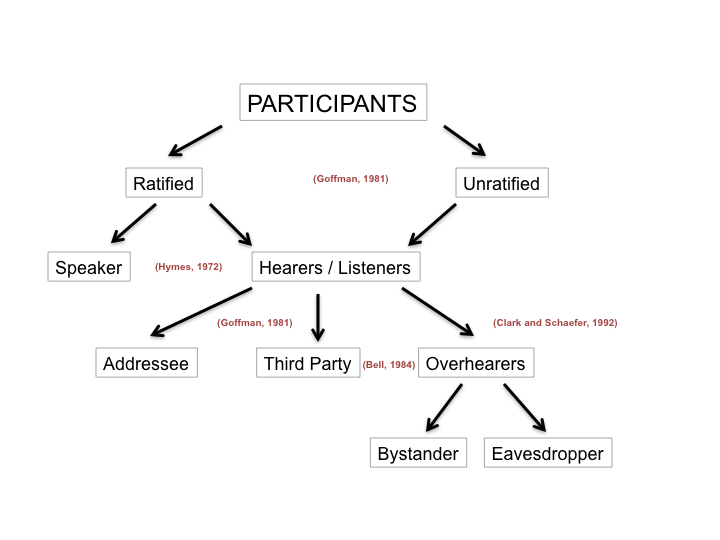
\includegraphics[scale=.75]{chapter7.tex/participants}
}
\caption{Modeling Hearers in Discourse (Adapted from  \citealp{Dynel:2010th})}
\label{participants}
\end{figure}

\begin{sloppier}
The distinction between bystanders and eavesdroppers serves an important distinction with respect to how speakers communicate. When the speaker is aware of a bystander, she can adjust her utterance in a number of ways. In dealing with overhearers, speakers  estimate how much the overhearer can infer; then design their utterances, accordingly \citep{Clark:1992ty}. 
\end{sloppier}

With respect to a shared common ground, there are two sorts of information that the speaker must consider. \textit{Open information} is information that overhearer believes or could readily guess to be in the common ground. \textit{Closed information} is information that the overhearer doesn't believe, and could not readily guess to be in the common ground \citep{Clark:1992ty}. It is the discrepancy between these two sorts of information that may be exploited by the speaker to affect what an overhearer (bystander or eavesdropper) might conjecture \citep{Clark:1992ty}. 

\begin{sloppier}
There are four main attitudes that a speaker can take toward overhearers: \textbf{indifference} (the speaker doesn't care whether the overhearer understands what she is saying or not), \textbf{disclosure} (the speaker tries to provide enough information that the overhearer can infer the right meaning), \textbf{concealment} (the speaker tries to deprive the overhearer of enough information to correctly infer what is meant --- e.g., you-know-who did you-know-what to whom), and \textbf{disguisement} (the speaker attempts to conceal her meaning from the observer while also deliberately mis-representing that meaning; \citep{Clark:1992ty}. 

Thus, \textbf{audience design} can be divided roughly into addressee design, third party design, and overhearer design \citep{Clark:1982tg}. It's worth noting that participant roles are constantly negotiated between interlocutors according to regular (e.g., turn-taking) procedures. And as \cite{Dynel:2010th} notes, one role may be performed by a number of individuals simultaneously.
\end{sloppier}

Online tracking represents a sort of discourse where the primary participants are a user interacting with a particular web site --- which has a participant role represented by a company or organization. Other hearers are present. Perhaps, ratified and perhaps not. When overhearers are not ratified, their understanding is not grounded. What they understand is conjecture. Sometimes what they may understand may be the same as a ratified hearer, and sometimes not. In an experiment conducted by \cite{Schober:1989wn}, ratified hearers were able to match understanding with the speaker with a very high degree of success. But despite the speaker and hearer deliberately obfuscating their speech in the presence of an overhearer, overhearers were still successful some of the time. More importantly, overhearers were also sometimes wrong.


\section{Aims}
\label{aims}

In this pilot, I consider whether experiment participants view advertisers as bystanders or eavesdroppers. To do this, I compare behavior across two conditions: subjects in the control condition answer a series of sensitive questions. In the treatment conditions, subjects perform the same task but are presented with visible evidence of advertisers as bystanders. This follows the general experiment design of  \citep{Acquisti:2012tp}  but poses a new dependent variable for investigation: \emph{visual presence}.

\section{Experimental Design}
\label{experimentaldesign}

This study has one experimental hypothesis:

\begin{description}
\item{Hypothesis 3} \hfill \\
People answering sensitive questions will behave differently in the presence of unratified participants than when simply notified in advance about the possibility of unratified participants.
\end{description}

In this \textbf{between} group, \textbf{single-factor}, \textbf{repeated measures} posttest-only design, the control group is asked to respond to a survey containing questions relating to sensitive activities (using questions drawn from  \cite{Acquisti:2012tp}).  Participants are notified in a privacy statement that there may be ad trackers on the site. The treatment group receives exactly the same notification and survey. However, tracker presence is indicated in a visual display throughout the participant's session. 

There is one \textbf{independent variable}: ``visual presence''. The \textbf{dependent variable} is the propensity to respond in affirmative to engaging in specific behaviors. This represents the willingness to divulge sensitive information under circumstances which may appear to be more or less private. 

Following presentation of stimuli, survey data is collected for both experimental designs. 

\section{Method}
\label{method}

This experimental design follow the general procedure outlined in Chapter Four.

\subsection{Settings and Participants}
\label{settingsandparticipants}

Using Amazon's Mechanical Turk, 213 workers were paid \$0.15 to participate in one of two conditions of the single-factor design previously described. Participants were assigned randomly via Qualtrics block randomizer. Results were collected during the period of 7--14 October 2014. The task was expected to take approximately three minutes, though workers were allowed up to 10 minutes to complete.

\subsection{Procedure and Materials}
\label{procedureandmaterials}

The general procedure follows that described in Chapter Four.  \autoref{3-flow}  is a more detailed graphical depiction of flow.

\begin{figure}
\centerline{
  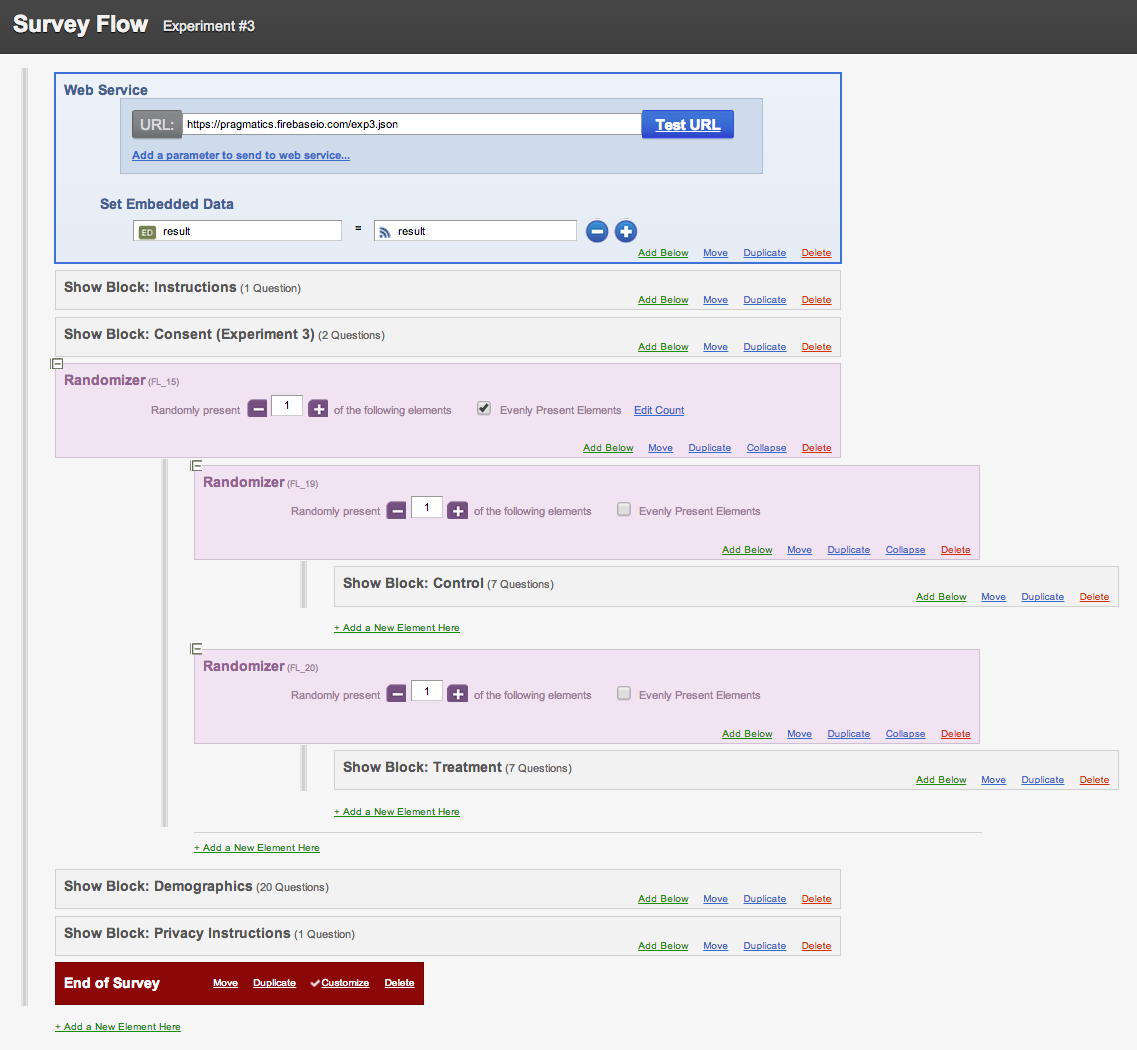
\includegraphics[scale=.3]{chapter7.tex/exp3-flow}
  }
\caption{Experiment 3 Flow}
\label{3-flow}
\end{figure}

Following presentation of instructions and consent form, participants were each presented the following six question in the order given.

\begin{enumerate}
\item Have you bounced a check?
\item Have you cheated on a tax return?
\item Have you made a false or even somewhat inflated insurance claim?
\item While an adult, have you had sexual desires for a minor?
\item Have you had sex with the current husband, wife, or partner of a friend?
\item Have you fantasized about having violent, non-consensual sex with someone?
\end{enumerate}

Possible answers were:

\begin{enumerate}
\item Never
\item Once or twice
\item Sometimes
\item Frequently
\end{enumerate} 

As in  \cite{Acquisti:2012tp},  propensity to disclose is indicated by a positive answer. All positive answers are combined into a single score. Non-answers (skipped questions) count as non-disclosure. Thus, the dependent variable is binary.

\subsection{Instrumentation}
\label{instrumentation}

In addition to features provided by AMT and Qualtrics, my scripts performed the following:

\begin{sloppier}
\begin{enumerate}
\item Disable preview using a custom CSS class blocking Qualtrics controls
\item Check worker hash against a FireBase web service and request worker to return HIT if the hash is in the exclusion list
\item Add worker hash to FireBase
\item Submit results to AMT on completion of the Qualtrics survey
\end{enumerate}
\end{sloppier}

No other instrumentation was required for this experimental design.

\section{Data Collected}
\label{datacollected}

Using a G* Power 3 f-test for linear multiple regression with a fixed model, I estimated a sample size of approximately 89 was necessary in order to detect a medium effect with power of 0.95. All surveys initiated were completed: there were no known drop-outs.

Once all assignments had been completed, (as indicated on my AMT requester dashboard), I downloaded data as a single CSV (comma separated values) file from the Qualtrics website. Data was organized such that each participant's data is on its own row.

\section{Results}
\label{results}

There is some difference in the demographic profile between the Experiment 3 sample and the  \citet{Acquisti:2012tp}  sample. That study reported a mean age of 40, 45\% male, and 82\% caucasian. This study was 63\% male, 82\% caucasian, 68\% under 35, and, likely, with lower income levels (given NYT has a subscription fee for regular readers): 53\% reportedly make below 30K. Regardless, comparing control group responses from  \cite{Acquisti:2012tp}  with control group responses here, propensity to disclose was very similar.

Interestingly, the percentage of male respondents for Experiment 3 was higher than the aggregate population studied across all experiments in this dissertation  (63\% versus 53\%; see \autoref{survey-response}).  This suggests that some population of workers, including females, elected not to participate in this study. I will come back to this point in a bit.

 \autoref{3-raw}  below presents averages across all six questions. A simple chi-square test reveals no difference between groups  (p = 1).\footnote{This is with and without a bonferroni adjustment for repeated questions (p = .046)} 


\begin{table}
\caption{Raw Results (Aggregate Mean)}
\label{3-raw}
\centering
\begin{tabular}{ccc}
\hline 
 & Control & Treatment\tabularnewline
\hline 
Never & 41.33 & 42.17\tabularnewline
Once or twice & 6.83 & 7.00\tabularnewline
Sometimes & 2.33 & 1.33\tabularnewline
Frequently & .50 & .50\tabularnewline
\end{tabular}\end{table}


There are two factors that may account for observed differences between this study and  \citet{Acquisti:2012tp}.  First, the population sampled here is surprisingly sensitive to privacy issues. Moreover, AMT as a platform is not seen as anonymous --- as the  \citet{Acquisti:2012tp}  survey may have been perceived. The mere fact that I presented an IRB form with names and contact information affected discourse context.

Second, answering specific questions in the  \cite{Acquisti:2012tp}  survey was completely voluntary; `no answer' accounted for between roughly 10--15\% for each question asked. This was calculated in the metric for propensity to disclose.

Selectional differences in this study are reflected in a couple of ways.

\begin{itemize}
 \item \textbf{Population Bias.} There is no way to know if the people who elected not to participate in Experiment 3 did so because they did not want to see "sensitive" questions or because they were concerned with privacy. Regardless, there is a population bias --- as reflected by the relative gender disparity between Experiment 3 and aggregate demographics across all five studies.
\item \textbf{Obligation.} No one in this experiment tried \textit{not} to answer a question. This may relate to the nature of the obligation workers feel to requesters as paid subjects. 
\end{itemize}


Over the course of the past two years, tremendous change has occurred on the Internet. Savvy users, like those found on AMT, are well aware that what they say and do may be monitored. One of my participants noted in comment, ``nothing is private online now due to the NSA.'' Events have conspired to raise the saliency of privacy issues on the Internet for even casual Internet users. Despite this, my survey reveals perceptual differences for feelings of privacy on the Internet whether connected at home or in a public setting. \autoref{privacy}  represents answers to the following two questions:

\begin{enumerate}
\item How private do you feel on the Internet when you are using your computer (laptop, or tablet) in public. Public means something like a coffee shop, library, school, etc.
\item How private do you feel on the Internet when you are using your computer (laptop, or tablet) at home?
\end{enumerate}

\begin{figure}
\centerline{
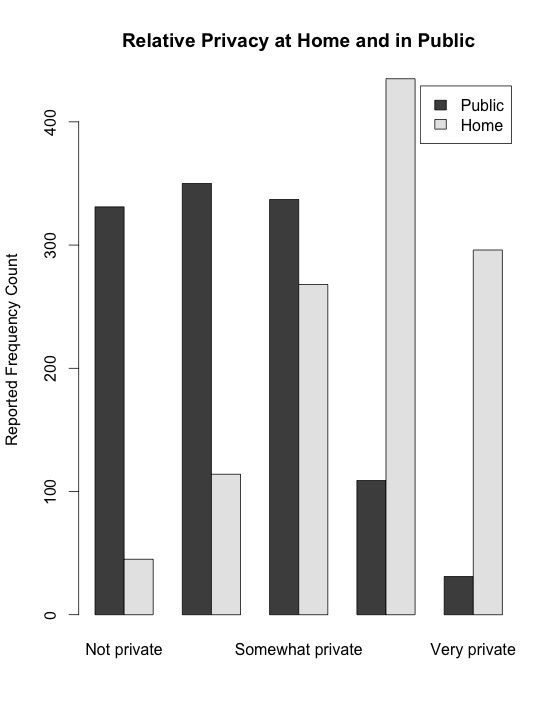
\includegraphics[scale=.5]{chapter7.tex/exp3-graph}
}
\caption{Feelings of Privacy on the Internet in Public and at Home}
\label{privacy}
\end{figure}

It's clear that physical setting, at least, lends some expectation of privacy whether one is on the Internet on a personal machine at home or in public. Though visual saliency was not a factor in propensity to disclose in this experiment, users have an expectation of privacy when they are not in a public setting. Given the Internet is now ``public'', there exists some mis-match of expectation that is not accounted for in Internet browser design.
